\section{Experiments}

\subsection{Setup}

All runs use OpenCLIP ViT-B/16 with LAION2B weights. The image and text encoders are frozen; only the adaptation modules are trainable. The selected R028 configuration uses $K=8$ residual channels, fixed residual gate $\alpha=0.05$, $\lambda_{\mathrm{anchor}}=10$, $\lambda_{\Delta}=0.01$, anchor ratio $0.75$, and no targeted relational loss. Remote jobs ran on RTX A6000 GPUs with no wandb logging.

The staged relation evaluation combines ARO/SugarCrepe-style relation and compositional counterfactual suites. Guardrail checks use COCO retrieval with 1,000 images and 5,002 captions, plus ImageNet zero-shot with 5,000 examples. External follow-ups use Winoground's 400 examples and Flickr30k retrieval with 1,000 images. The pilot gate used during experimentation required relation accuracy above the plain adapter, COCO image-to-text R@1 at least $0.70$, and ImageNet top-1 at least $0.55$.

The evaluation is organized by run families rather than isolated best checkpoints. R003 is frozen OpenCLIP. R005 is the plain adapter baseline. R011 and R014 are representative hard-token bottlenecks that replace the embedding path. R019, R025, and R027 are full RRB seed checks. R023, R028, R031, R032, and R035--R039 remove the targeted loss under different anchoring settings. R024 replaces structured relation counterfactuals with generic hard negatives. R033 and R040 remove the multi-channel bottleneck from the residual interface. R034, R041, R043, and R045 are follow-ups for external validity, mechanism, orthogonal projection, and Flickr30k retrieval.

The reported metrics are intentionally mixed. Relation accuracy measures the targeted failure mode, calculated as the simple average accuracy across all evaluated ARO and SugarCrepe sub-suites. COCO image-to-text R@1 measures whether the image embedding still retrieves the correct caption from a small held-out retrieval pool. ImageNet top-1 measures zero-shot category transfer. Residual magnitude and cosine-to-$\zbase$ summarize how much the adapted vector moves, but they are diagnostic rather than decisive. Winoground text, image, and group scores test a different binding setting, and Flickr30k checks whether the retrieval tradeoff transfers beyond the COCO guardrail split.

All numbers in this section come from the consolidated local experiment report and the copied remote-output summaries. The draft does not rerun the GPU training jobs during paper generation. That matters for interpretation: the paper is a faithful analysis of the existing run record, not a new benchmark campaign with exhaustive hyperparameter search.

% Auto-generated by figures/generate_paper_assets.py
\begin{table*}[t]
\centering
\caption{Main relation/anchor-preservation comparison. Relation accuracy is measured on staged ARO/SugarCrepe-style relation suites. COCO is image-to-text Recall@1 on the 1k-image guardrail split. Residual is the mean relative magnitude of the learned residual branch where available.}
\label{tab:main_results}
\small
\begin{tabular}{llrrrrrp{2.9cm}}
\toprule
Run & System & Relation & $\Delta$ vs R005 & COCO R@1 & ImageNet & Residual & Notes \\
\midrule
R003 & OpenCLIP & 0.6564 & -- & 0.7990 & 0.6670 & -- & Frozen OpenCLIP baseline \\
R005 & plain adapter & 0.6956 & 0.0000 & 0.7790 & 0.6438 & -- & Plain adapter baseline \\
R011 & hard token targeted & 0.7488 & 0.0532 & 0.3920 & 0.0660 & -- & Catastrophic guardrail degradation \\
R014 & hard token no targeted & 0.7332 & 0.0376 & 0.4110 & 0.0602 & -- & Catastrophic guardrail degradation \\
R019 & RRB full seed 1 & 0.7697 & 0.0741 & 0.7190 & 0.6152 & 0.1328 & Clears pilot guardrails \\
R028 & RRB no targeted, stronger anchor & 0.7734 & 0.0778 & 0.7340 & 0.6342 & 0.0804 & Selected configuration \\
R033 & no-slot residual adapter control & 0.7825 & 0.0869 & 0.3740 & 0.3308 & 0.2062 & Catastrophic guardrail degradation \\
R040 & constrained no-slot residual control & 0.7773 & 0.0817 & 0.4820 & 0.4798 & 0.0969 & Large retrieval/zero-shot degradation \\
\bottomrule
\end{tabular}
\end{table*}


\subsection{Main Tradeoff}

Table~\ref{tab:main_results} and Figure~\ref{fig:relation_coco} summarize the main tradeoff. In Figure~\ref{fig:relation_coco}, the selected configuration is highlighted with a star marker to distinguish it from other seed variations and baseline controls. OpenCLIP has the strongest broad guardrails among the core baselines, but lower relation accuracy. The plain adapter improves relation from $0.6564$ to $0.6956$ with a small guardrail tax. Hard token bottlenecks move relation further but collapse both guardrails: R011 reaches relation $0.7488$ with COCO R@1 $0.3920$ and ImageNet top-1 $0.0660$.

RRB demonstrates a distinct Pareto-style tradeoff compared with replacement bottlenecks. R019, the first full RRB seed, reaches relation $0.7697$ while passing the pilot COCO and ImageNet thresholds. The selected R028 checkpoint simplifies the method by removing the targeted loss and strengthening anchoring; it reaches relation $0.7734$, COCO R@1 $0.7340$, and ImageNet top-1 $0.6342$. This is still an alignment tax relative to OpenCLIP and the plain adapter, but it is not the catastrophic forgetting observed in the replacement bottlenecks.

The no-channel controls sharpen the interpretation. R033 reaches relation $0.7825$, higher than R028, but collapses COCO to $0.3740$ and ImageNet to $0.3308$. R040 constrains the same no-channel idea more strongly and reduces residual magnitude, but COCO remains only $0.4820$ and ImageNet $0.4798$. These controls show why relation accuracy cannot be optimized alone. They also support the architectural role of the multi-channel interface: a residual path without that bottleneck can find relation-improving directions that are incompatible with broad CLIP behavior.

The selected result is therefore a Pareto-style point, not a strict dominance claim. OpenCLIP and the plain adapter retain stronger retrieval. Some hard or unconstrained variants obtain relation scores close to or above R028. R028 is useful because it occupies a middle region that the earlier variants failed to reach: a substantial relation gain with retrieval and zero-shot scores still in a usable range. That is the paper's main empirical claim.

% Auto-generated by figures/generate_paper_assets.py
\begin{table}[t]
\centering
\caption{Structured counterfactuals, not the targeted relational loss $L_{targeted}$, explain the retained relation gain.}
\label{tab:ablation}
\small
\resizebox{\columnwidth}{!}{%
\begin{tabular}{llccrr}
\toprule
Run & Variant & Struct. CF & $L_{targeted}$ & Relation & COCO \\
\midrule
R023 & no-targeted, weak anchor & yes & 0 & 0.7922 & 0.6820 \\
R024 & generic hard negatives & no & 1 & 0.6736 & 0.7990 \\
R028 & selected stronger-anchor & yes & 0 & 0.7734 & 0.7340 \\
R029 & matched targeted control & yes & 1 & 0.7731 & 0.7280 \\
\bottomrule
\end{tabular}%
}
\end{table}


\subsection{What Training Signal Matters?}

Table~\ref{tab:ablation} separates structured counterfactual supervision from the targeted relational loss. R024 uses generic hard negatives rather than structured relational counterfactuals. It preserves COCO and ImageNet nearly perfectly, but relation accuracy drops to $0.6736$, below the plain adapter baseline. In contrast, R023 and R028 use structured counterfactuals with $L_{targeted}=0$ and retain large relation gains. R029 adds the targeted loss back under the same stronger-anchor setting and does not improve the selected tradeoff. The result is a useful anti-claim: the targeted loss sounded plausible but is not the supported mechanism.

This ablation is central because it prevents two overstatements. First, the gain is not explained by hard-negative training in general. If that were the explanation, R024 would have improved relation accuracy while preserving guardrails. It did the opposite: it preserved guardrails and lost the relation effect. Second, the gain is not evidence that targeted channel supervision discovers relation-specialized channels. R023 and R028 remove the targeted term entirely. R028 is the cleaner paper-facing method because it keeps the structured relation signal and the anchor terms while dropping a mechanism that the evidence does not need.

The R023/R028 comparison also shows why model selection cannot use relation accuracy alone. R023 reaches relation $0.7922$, higher than R028, but COCO falls to $0.6820$. R028 gives up some relation accuracy and passes the pilot guardrail. This tradeoff is exactly what the stronger anchor was meant to expose. The selected checkpoint is not the maximum relation model in the run history; it is the simplest relation-positive model that clears the explicit preservation gate.

% Auto-generated by figures/generate_paper_assets.py
\begin{table}[t]
\centering
\caption{Seed summaries for RRB variants. Values are mean $\pm$ sample standard deviation.}
\label{tab:seed_summary}
\small
\begin{tabular}{lrr}
\toprule
Group & Relation & COCO R@1 \\
\midrule
full RRB & 0.7768 $\pm$ 0.0062 & 0.6927 $\pm$ 0.0294 \\
anchor-10 no-targeted & 0.7782 $\pm$ 0.0042 & 0.7110 $\pm$ 0.0332 \\
anchor-20 no-targeted & 0.7789 $\pm$ 0.0032 & 0.7092 $\pm$ 0.0232 \\
\bottomrule
\end{tabular}
\end{table}


\subsection{Seed and Anchoring Stability}

\begin{figure}[t]
    \centering
    % Auto-generated by figures/generate_paper_assets.py
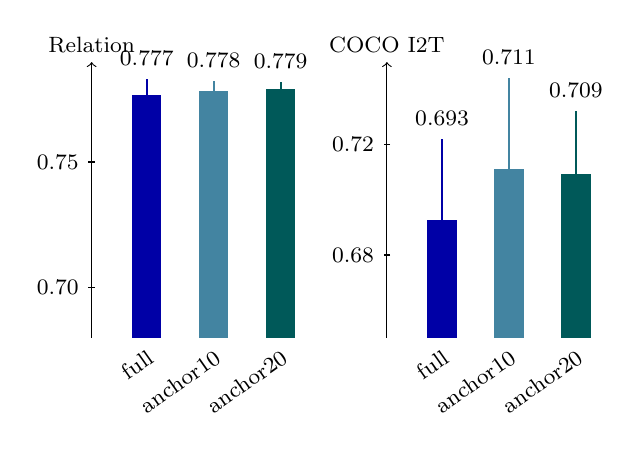
\begin{tikzpicture}[font=\footnotesize]
\draw[->] (0,0) -- (0,3.50) node[above] {Relation};
\draw[->] (3.75,0) -- (3.75,3.50) node[above] {COCO I2T};
\draw (0.04,0.64) -- (-0.04,0.64) node[left] {0.70};
\draw (0.04,2.23) -- (-0.04,2.23) node[left] {0.75};
\draw (3.79,1.05) -- (3.71,1.05) node[left] {0.68};
\draw (3.79,2.45) -- (3.71,2.45) node[left] {0.72};
\draw[fill=blue!65!black,draw=blue!65!black] (0.52,0) rectangle (0.88,3.08);
\draw[blue!65!black,thick] (0.70,2.88) -- (0.70,3.28);
\node[rotate=35,anchor=east] at (0.85,-0.15) {full};
\node[above] at (0.70,3.33) {0.777};
\draw[fill=blue!65!black,draw=blue!65!black] (4.27,0) rectangle (4.63,1.49);
\draw[blue!65!black,thick] (4.45,0.47) -- (4.45,2.52);
\node[rotate=35,anchor=east] at (4.60,-0.15) {full};
\node[above] at (4.45,2.57) {0.693};
\draw[fill=cyan!60!black,draw=cyan!60!black] (1.37,0) rectangle (1.73,3.13);
\draw[cyan!60!black,thick] (1.55,2.99) -- (1.55,3.26);
\node[rotate=35,anchor=east] at (1.70,-0.15) {anchor10};
\node[above] at (1.55,3.31) {0.778};
\draw[fill=cyan!60!black,draw=cyan!60!black] (5.12,0) rectangle (5.48,2.13);
\draw[cyan!60!black,thick] (5.30,0.97) -- (5.30,3.30);
\node[rotate=35,anchor=east] at (5.45,-0.15) {anchor10};
\node[above] at (5.30,3.35) {0.711};
\draw[fill=teal!70!black,draw=teal!70!black] (2.22,0) rectangle (2.58,3.15);
\draw[teal!70!black,thick] (2.40,3.05) -- (2.40,3.25);
\node[rotate=35,anchor=east] at (2.55,-0.15) {anchor20};
\node[above] at (2.40,3.30) {0.779};
\draw[fill=teal!70!black,draw=teal!70!black] (5.97,0) rectangle (6.33,2.07);
\draw[teal!70!black,thick] (6.15,1.26) -- (6.15,2.88);
\node[rotate=35,anchor=east] at (6.30,-0.15) {anchor20};
\node[above] at (6.15,2.93) {0.709};
\end{tikzpicture}

    \caption{Seed summaries show stable relation gains but imperfect COCO retention. Anchor-10 and anchor-20 no-targeted variants have similar mean COCO R@1 in these runs (0.711 and 0.709), so stronger anchoring does not eliminate retrieval performance degradation. Error bars are sample standard deviations.}
    \Description{Grouped summary chart comparing relation accuracy and COCO recall across full RRB, anchor-10 no-targeted RRB, and anchor-20 no-targeted RRB seed groups. Relation means are stable near 0.78, while COCO means vary and have nontrivial error bars.}
    \label{fig:seed_anchor}
\end{figure}

The seed summaries in Table~\ref{tab:seed_summary} and Figure~\ref{fig:seed_anchor} show stable relation gains and unstable retrieval retention. Full RRB over R019/R025/R027 has mean relation $0.7768 \pm 0.0062$, but mean COCO R@1 $0.6927 \pm 0.0294$, with only one of three runs clearing the COCO threshold. No-targeted anchor-10 runs R028/R031/R032 have mean relation $0.7782 \pm 0.0042$ and mean COCO $0.7110 \pm 0.0332$. Anchor-20 runs R035--R039 reduce residual drift in the consolidated diagnostics and keep relation stable, but their mean COCO remains $0.7092 \pm 0.0232$. The method therefore supports relation gains across seeds, not robust retrieval preservation across seeds.

The anchor-20 group is especially informative. It reduces mean residual magnitude to $0.0666$ and increases mean cosine-to-$\zbase$ to approximately $0.9975$, but this does not translate into a clearly higher COCO mean than the anchor-10 group. R038 is the best external-retrieval follow-up candidate in that group, yet other anchor-20 seeds still miss or nearly miss the COCO threshold. The result argues against a simple residual-size selection rule. Stronger anchoring can reduce drift, but relation-preserving directions and retrieval-preserving directions are not identical.

For a deployment-oriented paper, this would be a serious blocker. For this paper's more limited claim, it is part of the result. RRB gives a repeatable relation gain under multiple seeds and anchor settings, but retrieval preservation remains stochastic and incomplete. The right summary statistic is therefore not only the selected R028 point; it is the seed-group pass rate and variance around that point.

This is why the gate in Section~3.6 is a validation protocol rather than a guarantee. A relation-positive checkpoint is not considered usable until it also passes the COCO and ImageNet guardrails, and a run family is not considered stable unless its pass rate is reported. Under that stricter reading, R028 is evidence that a useful residual direction exists, while the seed table shows that the current training recipe does not find such directions reliably enough for deployment.

% Auto-generated by figures/generate_paper_assets.py
\begin{table*}[t]
\centering
\caption{External-validity and mechanism checks bound the claim. These follow-ups strengthen the limitation story rather than changing the main positive result.}
\label{tab:external_limits}
\small
\setlength{\tabcolsep}{3pt}
\begin{tabular}{p{2.1cm}p{4.1cm}p{7.7cm}}
\toprule
Check & Result & Interpretation \\
\midrule
\multicolumn{3}{l}{\textit{Downstream and external retrieval checks}} \\
Winoground R034 & R028 text/image/group 0.2400/0.1100/0.0700 vs OpenCLIP 0.2775/0.1075/0.0825 & Text and group scores drop while image score is nearly flat; no broad binding claim. \\
Flickr30k R045 & R028 I2T R@1 0.8260 vs OpenCLIP 0.8620; R038 0.8440 & External retrieval tax persists, smaller for anchor-20 R038. \\
\midrule
\multicolumn{3}{l}{\textit{Mechanistic and preservation probes}} \\
Slot responsibility R041 & entropy 1.0000, top-1 concentration 0.1259, edited overlap 0.1397 & Diffuse responsibility; no interpretable semantic-channel claim. \\
ROP ablation R043 & relation 0.7441, COCO 0.7360, ImageNet 0.6566 & Better preservation but relation gate fails; ROP remains an ablation/future direction. \\
\bottomrule
\end{tabular}
\end{table*}


\subsection{External Validity and Mechanism Checks}

Table~\ref{tab:external_limits} gives the boundary checks. Winoground does not support broad binding generalization: R028 scores $0.2400$ text, $0.1100$ image, and $0.0700$ group, while OpenCLIP scores $0.2775$, $0.1075$, and $0.0825$. Flickr30k confirms an external image-to-text retrieval tax: R028 drops from OpenCLIP's $0.8620$ to $0.8260$ I2T R@1, while R038 improves that to $0.8440$ but still does not match OpenCLIP. R041 responsibility probes are diffuse, with entropy near $1.0000$ and top-1 concentration near $0.126$, so the paper does not claim semantic channel specialization. R043's orthogonal-projection ablation preserves COCO and ImageNet better but fails the relation target, so it remains a cited ablation or future direction rather than a new headline.

The Winoground result is the cleanest warning against overgeneralization. R028 slightly improves image score by $0.0025$ over OpenCLIP but loses text and group score. A broad binding claim would require improvement on the group score, not only on staged ARO/SugarCrepe-style edits. The paper therefore treats Winoground as negative external-validity evidence. This is not surprising: the training signal emphasizes edited captions and margin ranking, while Winoground requires matching two captions and two images in a hand-curated setting where both visual and textual grounding must be correct.

Flickr30k gives a different warning. It is not a relation benchmark; it is an external retrieval distribution. The R028 image-to-text drop shows that the COCO guardrail is not a complete proxy for retrieval retention. R038 narrows the drop but does not close it. The text-to-image numbers are much closer to OpenCLIP, so an asymmetric retrieval tax is a plausible future-work hypothesis, not a claim established by the current small follow-up.

The responsibility probes close off the interpretability story. A useful semantic-channel result would show concentrated responsibility, consistent edited-token overlap, or stable channel assignments across examples. The observed entropy and top-1 concentration are close to diffuse. This does not invalidate the bottleneck as an architectural prior, but it does invalidate a stronger slot-semantics explanation. The final method name and captions therefore avoid promising interpretable slots.
